% id: 0214
% book: RPM 중3-2 수학 · 02 삼각비의 활용
% section: 유형 11 평행사변형의 넓이
% figure: crop:fig-0214.png
% answer: $15\sqrt{2}$
% answer_source: 답지
% variant_level: 0 (원본 전사)
% 이 파일은 build.mjs 가 items.json 에서 만든다. 고칠 때는 items.json 을 고친다.
\noindent\begin{minipage}[t]{0.58\linewidth}\vspace{0pt}\raggedright 오른쪽 그림과 같은 평행사변형~$\pt{ABCD}$에서 점~$\pt{M}$은 $\seg{BC}$의 중점이고 $\angle\pt{BAD}:\angle\pt{B}=3:1$일 때, $\triangle\pt{AMC}$의 넓이를 구하시오.\end{minipage}\hfill\begin{minipage}[t]{0.4\linewidth}\vspace{0pt}\centering \setlength{\dmfigw}{104.1pt}\ifdim\dmfigw>\linewidth\setlength{\dmfigw}{\linewidth}\fi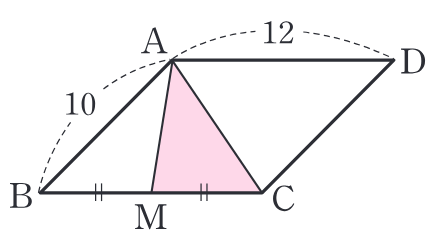
\includegraphics[width=\dmfigw]{figures/fig-0214.png}\end{minipage}\par
